\documentclass{article}
\usepackage[utf8]{inputenc}
\usepackage{amsmath}
\usepackage{tikz}
\usepackage[top=1in,right=1in,bottom=1in,left=1in]{geometry}
\usepackage{background}
\usepackage{booktabs} 
\usepackage{float}
\usepackage{listings}
\usepackage[linesnumbered,ruled]{algorithm2e}
\usepackage{enumerate}
\usepackage{graphicx}
\usepackage{parskip}
\usepackage{hyperref}

\SetBgContents{ }
\SetBgScale{1}
\SetBgAngle{0}
\SetBgOpacity{1}
\SetBgColor{black}
\SetBgPosition{current page.south west}
\SetBgHshift{3cm}
\SetBgVshift{1cm}

\title{CS 4780/5780 Homework 9 Solution\vspace{-10pt}}
\author{}
\date{}

\begin{document}
\maketitle

\section*{Problem 1: Convolutional-network}
	So here we construct Kernalization $\phi(x)$, which is a clever way to make inner products computationally tractable, so $$\phi(x)=\begin{bmatrix}
	h_{1}(x)\\
	.\\
	.\\
	.\\
	h_{m}(x)
	\end{bmatrix}$$ Each $h_{i}(x)$ is a linear classifier.
	(Not required)Here we draw the relationship among input $\vec{x}$, hidden layer $h_{m}(\vec{x})$ and output $H(\vec{x})$. Please see Figure \ref{fig:hw9_1}
	\begin{figure*}
		\centering
		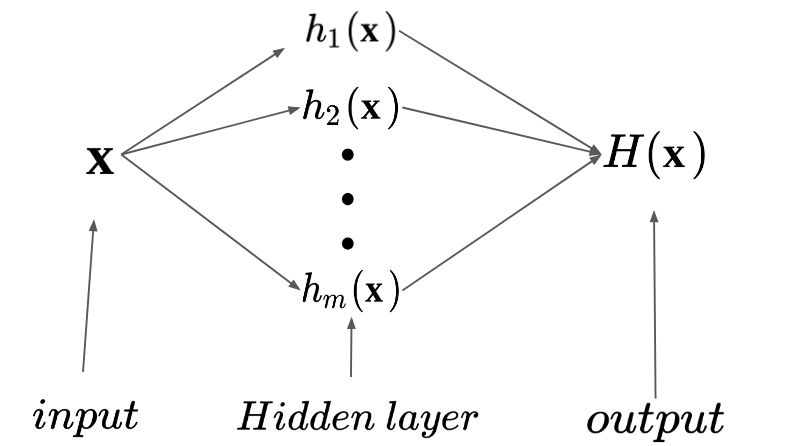
\includegraphics[width=5in,height=2.5in]{hw9_1.png}
		\caption{Neural Network}
		\label{fig:hw9_1}
	\end{figure*}
\section*{Problem 2: Convolutional Process}
\begin{enumerate}
	\item The dimension is $\frac{(n+2\times p -k)}{s}+ 1$
	\item The output is 
	 $$\begin{bmatrix}
	3&3 \\ 7 & 0  
	\end{bmatrix}$$
	
\end{enumerate}



\section*{Problem 3: RELU-network}
    \begin{enumerate}
        \item[(a)] To find the decision boundary, we will first express $\sigma(z)$ in terms of $x_1, x_2$. Using the weights and architecture given:

    \begin{align*}
        \begin{bmatrix} h_1 \\ h_2 \end{bmatrix} &= \begin{bmatrix} 1 & -1 & 0 \\ -1 & -1 & 0 \end{bmatrix} \begin{bmatrix} x_1 \\ x_2 \\ 1\end{bmatrix} \\
        h_1 &= x_1 - x_2 \\
        h_2 &= -x_1 - x_2
    \end{align*}

    \begin{align*}
        z &= \begin{bmatrix} 1 & 1 & -2 \end{bmatrix} \begin{bmatrix} f(h_1) \\ f(h_2) \\ 1 \end{bmatrix} \\
        &= f(h_1) +  f(h_2) - 2
    \end{align*}

    Putting this all together, we see that:

    \begin{align*}
        t &= \sigma(z) \\
        &= \sigma(f(h_1) + f(h_2) -2)\\
        &= \sigma(f(x_1 - x_2) + f(-x_1 - x_2) - 2) \\
        &= \frac{1}{1+e^{-(max(0, x_1 - x_2) + max(0, -x_1 - x_2) - 2)}}
    \end{align*}

    If you do this by hand, you can split the equation into the cases in which:
    \begin{itemize}
        \item $x_1 > x_2 ~ and ~ x_1 + x_2 > 0$
        \item $x_1 > x_2 ~ and ~ x_1 + x_2 < 0$
        \item $x_1 < x_2 ~ and ~ x_1 + x_2 > 0$
        \item $x_1 < x_2 ~ and ~ x_1 + x_2 < 0$
    \end{itemize}

    For all of these, you get the following equations:
    \begin{itemize}
        \item $\frac{1}{1+e^{-(x_1 - x_2 - 2)}}$
        \item $\frac{1}{1+e^{2(x_2 + 1)}}$
        \item $\frac{1}{1+e^{2}}$
        \item $\frac{1}{1+e^{x_1 + x_2 + 2}}$
    \end{itemize}

    Graphing this with Wolfram Alpha gives us:

    \begin{figure}[H]
        \centering
        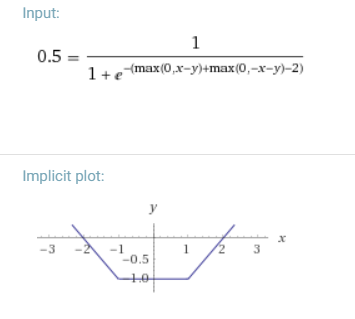
\includegraphics[width = 0.6\textwidth]{decision_boundary.png}
        \caption{Decision Boundary for the RELU Network}
        \label{fig:a}
    \end{figure}

    The top is classified negative, and the bottom is positive. (See Part B for more information.)

    \item[(b)] Plugging values into the equation from Part A, we see that the prediction for the point $\begin{bmatrix} 1 & 1 \end{bmatrix}^T$ is $\frac{1}{1+e^2} \approx 0.11920$. Since this is less than the decision boundary of 0.5, we classify this point as negative.

    \item[(c)] 
    Notice that $\frac{\partial t}{\partial z} = t(1-t)$ \\\\
    For i=1,2:
    $$
        \frac{\partial l}{\partial v_i} = \frac{\partial l}{\partial t} \cdot 
        \frac{\partial t}{\partial z} \cdot \frac{\partial z}{\partial v_3} = 
        (\frac{-y}{t}+\frac{1-y}{1-t}) \cdot (t \cdot (1-t)) \cdot f(h_i) = (t-y) \cdot f(h_i)    
    $$
    For i=3:
    \begin{align*}
        \frac{\partial l}{\partial v_3} = \frac{\partial l}{\partial t}\cdot\frac{\partial t}{\partial z}\cdot\frac{\partial z}{\partial v_3} = (\frac{-y}{t}+\frac{1-y}{1-t})\cdot(t\cdot(1-t))\cdot1 = t-y
    \end{align*}

    For j=1,2:
    \begin{align*}
        \frac{\partial l}{\partial w_{ij}} &= \frac{\partial l}{\partial t}\cdot\frac{\partial t}{\partial z}\cdot\frac{\partial z}{\partial f(h_i)}\cdot
        \frac{\partial f(h_i)}{\partial h_i}\cdot\frac{\partial h_i}{\partial w_{ij}} \\
        &= (\frac{-y}{t}+\frac{1-y}{1-t}) \cdot (t\cdot(1-t))\cdot v_i\cdot I(h_i>0)\cdot x_j \\
        &= (t-y)\cdot v_i\cdot I(h_i>0)\cdot x_j
    \end{align*}

    For j=3:
    \begin{align*}
        \frac{\partial l}{\partial w_{i3}} &= \frac{\partial l}{\partial t} \cdot \frac{\partial t}{\partial z} \cdot \frac{\partial z}{\partial f(h_i)}\cdot
        \frac{\partial f(h_i)}{\partial h_i} \cdot \frac{\partial h_i}{\partial w_{i3}}\\
        &= (\frac{-y}{t}+\frac{1-y}{1-t}) \cdot (t\cdot(1-t))\cdot I \cdot I(h_i>0) \cdot 1 \\
        &= (t-y)\cdot v_i \cdot I(h_i>0)
    \end{align*}
\end{enumerate}






\end{document}
